%\documentclass[JIP,draft]{ipsj}
\documentclass[JIP]{ipsj}

\usepackage[dvips]{graphicx}
\usepackage{latexsym}
\usepackage{amsmath}

\def\Underline{\setbox0\hbox\bgroup\let\\\endUnderline}
\def\endUnderline{\vphantom{y}\egroup\smash{\underline{\box0}}\\}
\def\|{\verb|}

%\setcounter{volume}{20}% vol20=2012
%\setcounter{number}{4}% 1, 2, 3, 4
\setcounter{page}{1}

%\received{2011}{7}{1}
%\rereceived{2011}{10}{1}   % optional
%\rerereceived{2011}{10}{31} % optional
%\accepted{2011}{11}{5}

\usepackage[varg]{txfonts}%%!!
\makeatletter%
\input{ot1txtt.fd}
\makeatother%

\begin{document}

\title{Relaxing CDN Energy: Considering Peer-Assisted}

\affiliate{SFC}{Keio University Shonan Fujisawa Campus, 5322 Endo, Fujisawa-shi, Kanagawa 252-0882 Japan}

\author{Mohamad Dikshie Fauzie}{SFC}[dikshie@sfc.wide.ad.jp]
\author{Achmad Husni Thamrin}{SFC}[husni@ai3.net]
\author{Jun Murai}{SFC}[jun@wide.ad.jp]


\begin{abstract}
This paper presents an analysis of a peer-assisted CDN system, where an ISP manages its own CDN and its users participate in a P2P network to assist content delivery.
The system consists of a two-level CDN, where one level can be considered as the current CDN and the other level is managed by the ISP, and a number of user nodes forming a P2P network, where some of the user nodes are obliged to contribute in the content delivery.


\end{abstract}

\begin{keyword}
CDN, Data Center, Energy, Peer Assisted, P2P
\end{keyword}

\maketitle

%1
\section{Introduction}\label{intro}
Streaming content, especially video, represents a significant fraction of the traffic volume on the Internet, and it has become a standard practice to deliver this type of content using Content Delivery Networks (CDNs) such as Akamai and Limelight for better scaling and quality of experience for the end users.  
For example, Youtube uses Google cache and MTV uses Akamai in their operations.

With the spread of broadband Internet access at a reasonable flat monthly rate, users are connected to the Internet 24 hours a day and they can download and share multimedia content.  
P2P (peer to peer) applications are also widely deployed.  
In China, P2P is very popular; we see many P2P applications from China such as PPLive, PPStream, UUSe, Xunlei, etc.  
Some news broadcasters also rely on P2P technology to deliver popular live events.  
For example, CNN uses the Octoshape solution that enables their broadcast to scale and offer good video quality as the number of users increases.

From the Internet provider point of view, the presence of so many always-on users suggests that it is possible to delegate a portion of computing, storage and networking tasks to the users, thus creating P2P networks where users can share files and multimedia content.
Starting from file sharing protocols, P2P architectures have evolved toward video on demand and support for live events.

Broadband network access helps P2P applications to perform better.
xDSL networks are deployed worldwide, and in some countries, such as Japan, even higher bandwidth fiber to the home (FTTH) already exceeds DSL in market penetration.  In the coming years, FTTH will be massively deployed by network operators throughout the world.  
As access bandwidth increases, P2P systems may become more efficient since a peer can contribute much more.

On the other hand, data center where CDN server placed faces costs for powering the data center.
The Uptime Institute, a global data center authority, surveyed 1100 data center owners and operators on 2012, reported that 55\% organizations must increase budget 10\% than 2011 \cite{uptime}.  
30\% of organizations will run out of data center capacity (power, cooling, space, and network) in the end of 2012 \cite{uptime}. 
More than 50\% organizations surveyed reported that saving energy is major priority \cite{uptime}.
The increases in energy cost and the demand due to growth of traffic urges the data center operators and owners to look for ways to reduce energy usage in the years to come.
Although reducing energy consumption can effectively reduce overall cost, this will limit the capacity growth and scalability of the service provisioning.
Alternatively, the data center and be revamped by relocating some services to end-host computers or peers.
Peers contribute their communication, storage, and computation resources to exchange data and provide services while the data center performs central administration and authentication as well as backend processing.
P2P network, formed by peers offer flexibility and scalability in service delivery.
Therefore, P2P services can assist and enhance data center.
It is not our aim to advocate one system architecture over another.
Many issue such as manageability, reliability, and ease of deployment must be taken into account when making high level architectural decisions.

In this paper, we study the energy consumption of hybrid CDN-P2P.  
It has been known that CDN energy consumption is better than P2P architecture, unfortunately that model only think small part of problem energy consumption (devices/hardwares).
To be fair, we also need to change paradigm that to see if we also can relax power budget of data center by utilizing P2P.   
If we can move part of computation resource from CDN in data center to P2P, then we can relax power budget of data center for hardware dan cooling. 

The rest of this paper is organized as follows. Section 2 provides an overview of system model, data center model and energy model.  
In section 3, we will present result and analysis.  
Section 4 will conclude this paper. 

\begin{figure}[tb]
\begin{center}
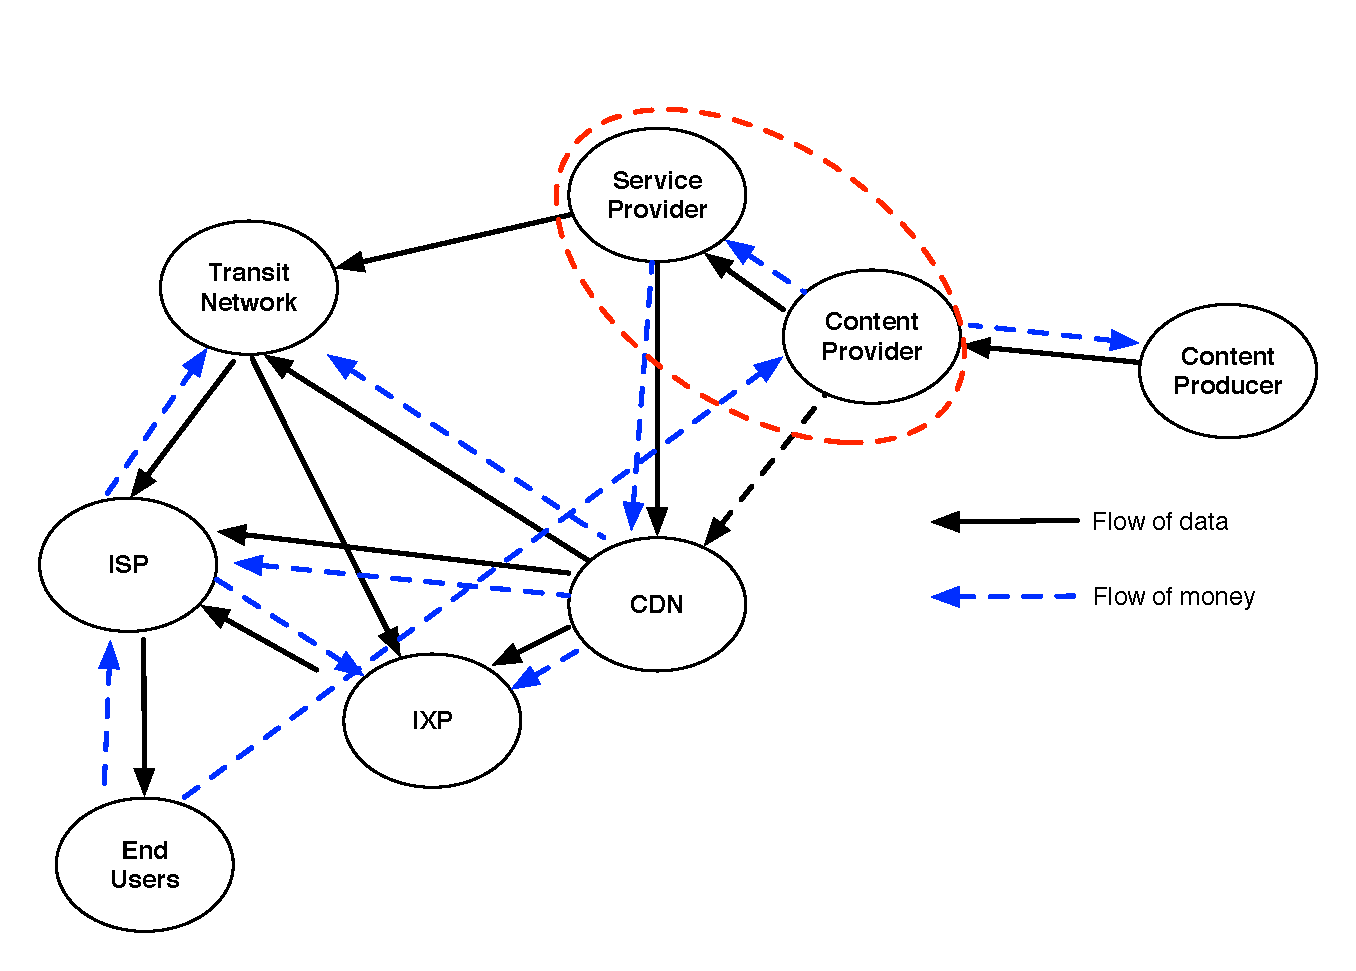
\includegraphics[scale=0.4]{graphs/business-relationship.eps}
\end{center}
\caption{In Complex relationship of entities in Internet, 
CDN mostly placed in data center near to eyeball ISP. 
If CDN can not reach eyeball ISP due to business or economic reason, CDN can be placed near to IXP or even inside IXP, and CDN will reach eyeball ISP from peering point inside IXP.}
\label{fig:businessrelationship}
\vspace{-2mm}
\end{figure} 

\section{Motivation}\label{motivation}
In the economic supply chain of video traffic, most ISPs get a little revenue from video traffic thus ISP wants to monetize that traffic.
the future of CDN business is likely to live deeper into ISP networks, more integrated into and interleaved with ISP infrastructures thus users can get good quality of video.
The idea of ISP managed CDN has been proposed in recent years.
The complexity of the CDN business encourage ISP to manage their own CDN rather than allow others to run CDNs on their networks.

CDN architectures are host-oriented: content is delivered to end users through host servers that are centrally managed in a few data centers fig.\ref{fig:businessrelationship}. 
The growing of Internet traffic dominated by video, the energy consumption of a host oriented architecture becomes problematic due to over provisioning factor.
The idea of utilizing the user's computation power to support ISP operation is not new. 
The figaro project proposed residential gateway as an integrator of different networks and services, becoming an Internet wide distributed content management for a proposed future Internet architecture.  
In this case, ISP can offload part of workload on their CDN to user's home gateway.  
By offloading workload, their CDN can relax energy demand thus relaxing data center power budget or relaxing capacity planning for power.





\section{System Description}\label{system model}
\begin{figure}[thb]
\begin{center}
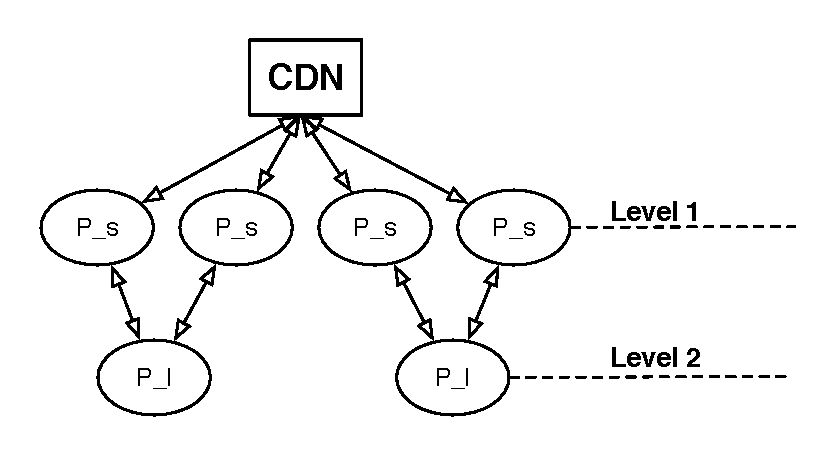
\includegraphics[scale=0.5]{graphs/p2p-cdn.eps}
\end{center}
\caption{A typical content delivery architecture with peer assisted.}
\label{fig:iptv}
\vspace{-2mm}
\end{figure} 

Figure \ref{fig:iptv} shows typical CDN with peer assisted.  
$P_s$ in fig.\ref{fig:iptv} is peers in level 1 or seeders.  
Seeders get content directly from CDN.  
$P_l$ in fig.\ref{fig:iptv} is peers in level 2 or leechers.
Leechers get content from seeders.
Maximum number of seeders is bounded by maximum CDN's capacity, while maximum number of leechers in level 2 is bounded by number of seeders can support the bitrate.
Denote number of seeders is $n_s$, number of leechers is $n_l$, $\rho$ is maximum bitrate that supplied by seeders to leechers, and $r=1$ is video bitrate, therefore we have number of leechers that can be supported by seeders is:

\begin{equation}\label{eqn:leecher}
	\lfloor n_l \rfloor = n_s . \rho
\end{equation}

Number of seeders that support or upload content to leecher is:

\begin{equation}\label{eqn:seeders-to-leechers}
	n_{s}^{u} = n_l . \frac{r}{\rho}
\end{equation}

The illustration as follows, suppose we have video bitrate $r=1$, seeder upload rate $\rho=0.25$, and maximum CDN capacity is $643Mbps$. 
Maximum number of seeders supported by CDN is $n_s=643$.
Maximum number leechers supported by seeders is $n_l=160$.  
Number of seeders that upload content to leechers is $n_{s}^{u}=640$.  
Therefore we have three seeders that do not need to upload content to leecher. 


\subsection{Thermodynamics of Data Center}\label{thermodynamics}
\begin{figure}[thb]
\begin{center}
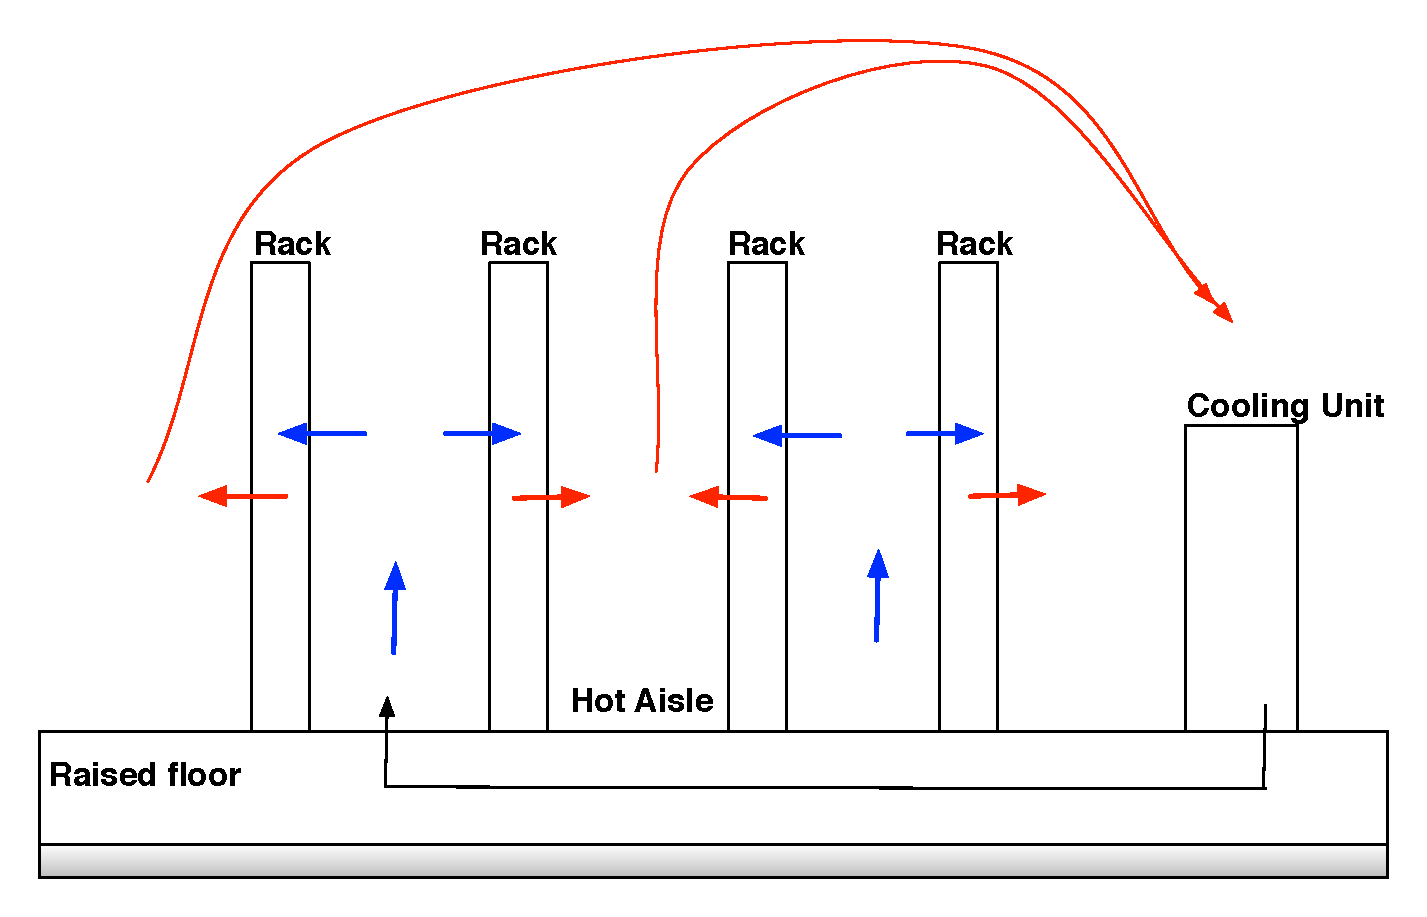
\includegraphics[scale=0.3]{graphs/datacenter.eps}
\end{center}
\caption{A typical data center schematic.
The cooling infrastructure comprises industry standard racks on a raised floor, through which multiple compressor-driven computer room air conditioning unit circulate cool air through a share plenum.}
\label{fig:datacenter}
\vspace{-2mm}
\end{figure} 
Many aspects of thermodynamics involved in data center.  
In this section, we only focus on relationship between cooling power and hardware temperature.

Data center seek to provision the cooling adequately to extract the heat produce by servers, switches, routers, and other devices.
Practically, cooling provisioning are done at facilities level.
Data center operator operate cooling facilities based on power ratings of servers, switches, routers, and other devices often with some additional headroom for risk tolerance. 
The compounded over provisioning of computing and cooling infrastructures can drive up initial and recurring costs. 

The cooling cycle of a typical data center operates in the following way:
Cooling units operate by extracting heat from the data center and pumping cold air into the room, usually through a pressurized floor plenum.
The pressure forces the cold air upward through vented tiles, entering the room in front the hardware
Fans draw the cold air inward and through the server; hot air exits through the rear of the server.
The hot air rises sometimes with the aid of fans and a ceiling plenum , and is sucked back to the cooling units.
The cooling units force the hot air past pipes containing cold air or water. 
The heat from the returning air transfer through the pipes to the cold substance. 
The heated substance leaves the room and goes to a chiller and cooling unit fans force the cold air back into the floor plenum. 
Above process is shown in fig.\ref{fig:datacenter}

The efficiency of this cycle depends on several factors, including the conductive substance and the air flow velocity, but it is quantified by coefficient of performance (COP).
The COP is the ratio of heat removed ($Q$) to the amount of work necessary ($W$) to remove that heat:

\begin{equation}\label{eqn:cop}
	COP=\frac{Q}{W}
\end{equation}

Therefore, the work necessary to remove heat is inversely proportional to the COP.  
A higher COP indicates a more efficient process, requiring less work to remove a constant amount of heat.

However, the COP for a cooling cycling is not constant, increasing with the temperature of the air the cooling unit pushes into the plenum.  
COP value empirically can be computed using \cite{moore2005making}:

\begin{equation}\label{eqn:copt}
	COP(T) = 0.0068.T^2 + 0.0008.T + 0.458
\end{equation}

where $T = T_{sup} + T_{adj}$ and $T_{adj} = T_{safe}^{in}-T_{max}^{in}$. \\
$T_{sup}$ is temperature supply by cooling unit and $T_{adj}$ is temperature difference between maximum safe hardware inlet temperature ($T_{safe}^{in}$) and the maximum observed hardware inlet temperature ($T_{max}^{in}$).
If $T_{adj}$ is negative, it indicates that a hardware inlet exceeds maximum safe temperature thus we need to lower $T_{sup}$ to bring the hardwares back below the system redline level.

\begin{figure}[thb]
\begin{center}
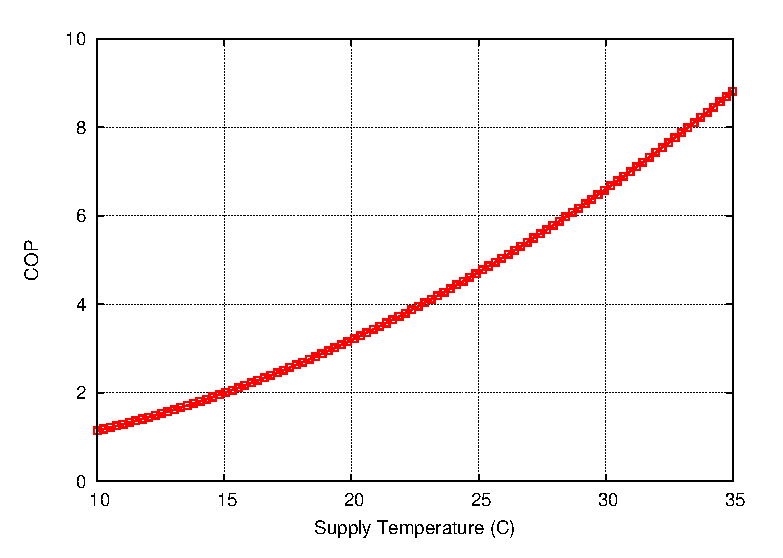
\includegraphics[scale=0.4]{graphs/cop.eps}
\end{center}
\caption{COP curve for the chilled water cooling units from HP Lab utility data center.
As the target temperature of the air the cooling unit pumps into the floor plenum increases, the COP increases.}
\label{fig:twotier}
\vspace{-2mm}
\end{figure} 

Cooling cost can be calculated as  \cite{moore2005making} :

\begin{equation}\label{eqn:cost}
C = \frac{Q}{COP(T)}
\end{equation}

Where $Q$ is amount of power the servers and hardwares consume.
COP(T) is our COP at $T=T_{sup}+T_{adj}$.
Currently we assume a uniform $T_{sup}$ from each cooling units due to the complications introduced by non-uniform cold air supply.


\subsection{Energy Model}\label{energy model}
In this paper, our goal is to provide a general view and a fair comparison of the energy consume by a CDN and hybrid CDN-P2P architecture. 
To do so, we designed a series of model and perform an analysis.
Our energy model is similar to the models used in \cite{Nedevschi:2008:HDC:1855610.1855618}.
Network model for energy is assumed to be flat network as shown in fig.\ref{fig:iptv}.

The energy consumption for a single request in data center as:
\begin{equation}
	E_{d} = E_s
\end{equation}

while the energy consumption for a single request in network as:
\begin{equation}
	E_{d} = d.E_r
\end{equation}

where $d_s$ is number of hops or the path length.

We introduce the notion of the energy consumed per bit transferred by each servers and routers then measure the per-request consumption by multiplying the per bit consumption with number of bits transferred per request.  
We define $\delta_s$ and $\delta_r$ work-induced energy consumed per additional bit transferred by a server and router.   
We also define $\gamma_s$ and $\gamma_r$ is the baseline energy consumed per processed bit.  
We can express these per-bit work induced consumptions as follows:
\begin{equation}
	\delta_s = \frac{(S_{max} - S_{base})}{M_s} 
\end{equation}
$S_{base}$ is a server's baseline power consumption.  
$S_{max}$ is a server's power when operating at maximum capacity.
$M_s$ is the maximum capacity in bit per second for a server.
Same formulation also applied for router.  
\begin{equation}
	\delta_r = \frac{(R_{max} - R_{base})}{M_R} 
\end{equation}
$R_{max}$ is a router power when operating at maximum capacity.
$R_{base}$ is a router's baseline power consumption.
$M_R$ is maximum capacity in bit per second for a router.

For baseline energy consumption, we expressed as: 
\begin{equation}
\begin{split}
	\gamma_s &= \frac{S_{base}}{\mu_s.M_s} \\
	\gamma_r &= \frac{R_{base}}{\mu_r.M_R}
\end{split}
\end{equation}
$\mu_s$ and $\mu_r$ is the average utilization at a server and a router.
We summarize the notation of the key parameters and its value in table.\ref{tab:parameters}.

\begin{table}[tb]
\caption{Notation of Key Parameters and Its Value from \cite{Nedevschi:2008:HDC:1855610.1855618}.}
\label{tab:parameters}
\hbox to\hsize{\hfil
\begin{tabular}{l|l}\hline\hline
Symbol & Value\\\hline
$\delta_s$ & $5.2 . 10^{-8}$ (J/b)\\
$\gamma_s$ & $6.7 . 10^{-7}$ (J/b)\\
$\delta_r$ & $8.0 . 10^{-9}$ (J/b)\\
$\gamma_r$ & $1.5 . 10^{-7}$ (J/b)\\\hline
\end{tabular}\hfil}
\end{table}



Considering cooling energy, we can rewrite:  




We also considering content popularity distribution.   
We assume that content provider has a content catalog of size $F$, ranked from 1 to $F$ based on popularity.   
$1$ represents the most popular content.
Letting the total number of requests in a given time duration $t$ will be $R$, the number of requests for content of popularity $k$, $R_k$ follows Zipf distribution as:

\begin{equation}
	R_k = R \frac{k^{-\beta}}{\sum_{k=1}^F k^{-\beta}}
\end{equation}

A large $\beta$ indicates a relatively small set of very popular content.
Typical value of $\beta$ range between $0.5$ and $1.0$.
IPTV channel has $\beta=0.8$ \cite{Cha:2008:NTP:1855641.1855646}.






\section{Result and Analysis}\label{analysis}


\section{Related Work} 

Content Distribution Networks with peer assist have been successfully deployed on the Internet, such as Akamai \cite{Huang:2008:UHC:1496046.1496064} and LiveSky \cite{Yin:2010:LEC:1823746.1823750}.  
The authors of \cite{Huang:2008:UHC:1496046.1496064} conclude from two real world traces that hybrid CDN-P2P can significantly reduce the cost of content distribution and can scale to cope with the exponential growth of Internet video content.  
Yin et al. \cite{Yin:2010:LEC:1823746.1823750} described commercial operation of a peer-assisted CDN in China.  
LiveSky solved several challenges in the system design, such as dynamic resource scaling of P2P, low startup latency, ease of P2P integration with the existing CDN infrastructure, and network friendliness and upload fairness in the P2P operation.  
Xu et al.\cite{DBLP:journals/corr/abs-1212-4915} using game theory, showed that the right cooperative profit distribution of P2P can help the ISP to maximize the utility.  
Their model can easily be implemented in the context of current Internet economic settlements.  
Misra et al.\cite{Misra:2010:IPS:1811099.1811064} also mentioned the importance of P2P architecture to support content delivery networks.
The authors use cooperative game theory to formulate simple compensation rules for users who run P2P to support content delivery networks.

The idea of telco- or ISP-managed CDN has been proposed in recent years.  
The complexity of the CDN business encourage telcos and ISPs to manage their own CDN, rather than allow others to run CDNs on their networks.  
It has been shown that it is cost effective \cite{federation}\cite{norton2011internet}. 
Kamiyama et al. \cite{NoriakiKAMIYAMA2013} proposed optimally ISP operated CDN.
Kamiyama et al. mentioned that, in order to deliver large and rich Internet content to users, ISPs need to put their CDNs in data centers.  
The locations are limited while the storage is large, making this solution effective, using optimum placement algorithm based on real ISP network topologies.  
The authors found that inserting a CDN into an ISP's ladder-type network is effective in reducing the hop count, thus reduce total link cost.  
Cisco has initiated an effort to connect telco- or ISP-managed CDNs to each other, to form a CDN federation \cite{federation} using open standards \cite{cdni}.  
They argue that the current CDN architecture is not close enough to the users and ISPs can fill this position.

The idea of utilizing the user's computation power to support ISP operation is not new.  The Figaro project \cite{figaro} proposed residential gateway as an integrator of different networks and services, becoming an Internet-wide distributed content management for a proposed future Internet architecture \cite{figaro}.  
Cha e al.,\cite{Cha:2008:NTP:1855641.1855646} performed trace analysis and found that an IPTV architecture powered by P2P can handle a much larger number of channels, with limited demand for infrastructure compare to IP multicast.  
Jiang et al. \cite{Jiang:2012:OMD:2413176.2413193} proposed scalable and adaptive content replication and request routing for CDN servers located in users' home gateways.  
Maki et al.\cite{NaoyaMAKI2012} propose traffic engineering for peer-assisted CDN to control the behavior of clients, and present a solution for optimizing the selection of content files.
Mathieu et al., \cite{6249305} are using data gathered from France telecom network to calculate reduction of network load if customers are employed as peer-assisted content delivery.
Our work is same in system model architecture which uses different level of topologies  (Level-0 and Level-1), where in Mathieu et al., \cite{6249305} the authors use different names, which are regional and national. 
We emphasize that compare to  Mathieu et al., \cite{6249305} our work provides completely different approach.
Mathieu et al., \cite{6249305} work mostly based on empirical data from France telecom company thus the authors can directly calculate network load caused by video traffic and calculate network load reduction if peer-assisted is employed on customers side,  while our study focus on mathematical model of different admission policies for peers to join peer-assisted CDN and ISP payoff can get from employing peer-assisted CDN.


\section{Conclusion and Future Work}\label{conclusion}

This paper presents a scheme for a ISP managed peer-assisted CDN model that estimates lower bound of peers based on a stochastic fluid model and estimate the economic incentive for ISP based on game theory.
While a higher upload rate from the user nodes acting as seeders is desirable, it should be noted that an ISP should be aware of the implication that offering an economic incentive to too many users in order to get them acting as seeders in the P2P would have an undesirable effect on the ISP's revenue.
Some areas of improvement that we have identified for future are:
more work on the stochastic fluid model to include multiple video streaming bitrate and downtime effect of user home gateway and penalty to ISP payoff. 
We are also very interested to include energy trade off this peer-assisted CDN architecture in order to know how much energy saving by ISP and how much increase of energy at users home gateway side in this architecture.


\begin{acknowledgment}
We thank Rodney Van Meter for suggestions.
\end{acknowledgment}

\bibliographystyle{ipsjunsrt-e}% bib style
\bibliography{journal}% your bib database



\begin{biography}

\profile{Mohamad Dikshie Fauzie}{was born in 1976.\
He received a bachelors degree and a master's degree from Institute of Technology Bandung, Indonesia.\
He is currently a Ph.D candidate at Keio University's Shonan Fujisawa Campus.}
%
\profile{Achmad Husni Thamrin}{is Assistant Professor at Keio University.\ 
He is a graduate of Keio University, Graduate School of Media and Governance (Ph.D 2005, MMG, 2002).\
His research interests include multicast, Internet over broadcast media, and peer-to-peer networks.} 
%
\profile{Jun Murai}{was born in March 1955 in Tokyo.\
Graduated Keio University in 1979, Department of Mathematics, Faculty of Science and Technology.\
He received his M.S. for Computer Science from Keio University in 1981,
and received his Ph.D. in Computer Science, Keio University in 1987.\ 
He specializes in computer science, computer network, and computer 
communication. He is currently Dean of the Faculty of Environment and Information Studies, Keio University since October 2009.\
Former Vice-President of Keio University from May 2005 to May 2009.\ 
He was an Executive Director of the Keio Research Institute at SFC, Keio University from 1999 to 2005.}
%
\end{biography}
\end{document}
